\documentclass{beamer}
\usepackage[utf8]{inputenc}
\usepackage[T2A]{fontenc}    
\usepackage[english,russian]{babel} 
\usepackage{graphicx}

\title{Лабораторная работа №7 по информатике (dop)}
\author{Ovsyannikov Roman Dmitrievich P3112}
\institute{Вариант 7}
\date{November 2021}

\begin{document}
\frame{\titlepage}


\begin{frame}
\frametitle{Современные языки разметки}
\center{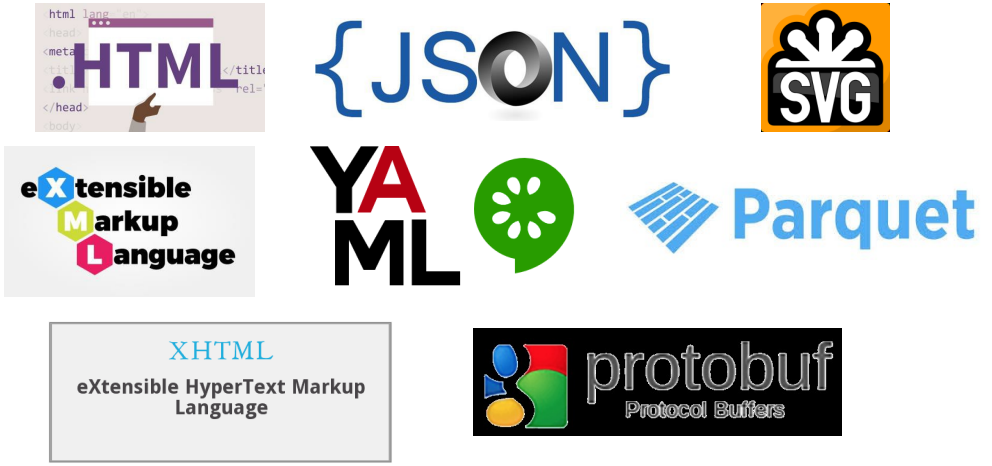
\includegraphics[scale=0.4]{dpic}}
\end{frame}

\begin{frame}
\frametitle{Примеры из жизни}
{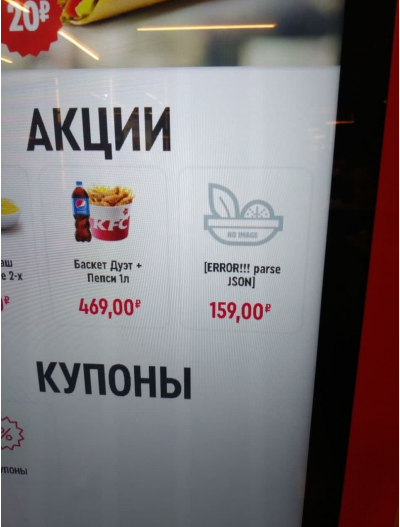
\includegraphics[scale=0.6]{dpic3}}
{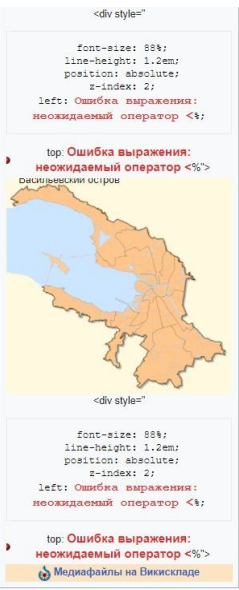
\includegraphics[scale=0.6]{dpic2}}
\end{frame}

\begin{frame}
\frametitle{Примеры из жизни (2)}
{
\includegraphics[scale=0.6]{dpic5}}
\begin{minipage}[c]{6cm}

\includegraphics[scale=0.6]{dpic4}
\end{minipage}
\begin{minipage}[c]{4cm}
Viber: JSON\\
WhatsApp: JSON\\
Telegram: TL(Type Languare,\\
собственный ML телеграма)/JSON\\
VK: JSON\\
Twitter: JSON
\end{minipage}
\end{frame}

\begin{frame}
\frametitle{Markdown}
\center{Markdown — облегчённый язык разметки.}
{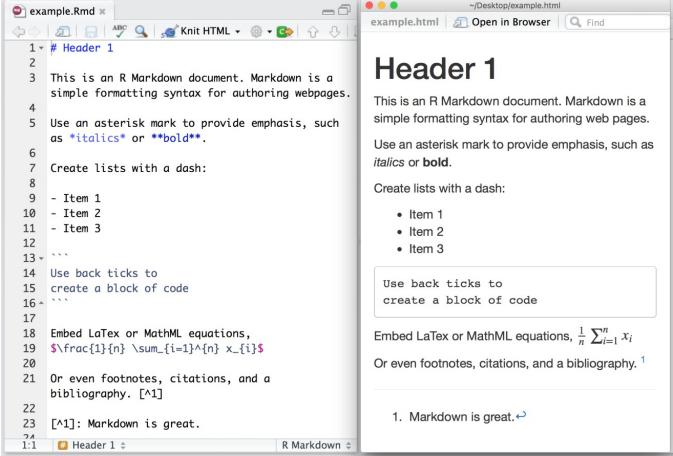
\includegraphics[scale=0.6]{dpic6}}
\end{frame}

\begin{frame}
\frametitle{Полезные ссылки}
\center{https://typora.io/ - Рекомендуемый многими Markdown-редактор\\
https://dillinger.io/ - Markdown online\\
https://jsonformatter.org/ - JSON online парсер\\
http://yaml-online-parser.appspot.com/ - YAML online parser\\
https://www.pvsm.ru/java/70568/ - Сравнение JSON и YAML\\
https://habr.com/post/248147/ - Сравнение XML, YAML и JSON\\
https://habr.com/company/wrike/blog/279797/ - Parquet\\
https://wtools.io/ - Удобный конвертор между форматами\\
https://onlinejsontools.com/ - Ещё один конвертор}
\end{frame}



\end{document}